\documentclass{beamer}
\usepackage[spanish]{babel}
\usepackage[utf8]{inputenc}
\usepackage{amsmath, amssymb, amsfonts}

\usetheme{Madrid}
\usecolortheme{default}
\useinnertheme{circles}

\definecolor{Logo1}{rgb}{0.208, 0.2865, 0.373}
\definecolor{Logo2}{rgb}{0.000, 0.674, 0.863}

\setbeamercolor*{palette primary}{bg=Logo1, fg=white}
\setbeamercolor*{palette secondary}{bg=Logo2, fg=white}
\setbeamercolor*{palette tertiary}{bg=white, fg=Logo1}
\setbeamercolor*{palette quaternary}{bg=Logo1,fg=white}
\setbeamercolor{structure}{fg=Logo1} % itemize, enumerate, etc
\setbeamercolor{section in toc}{fg=Logo1} % TOC sections

%------------------------------------------------------------
% Este bloque de código define la información que aparecerá en la página de título.
\title[Criterios de Convergencia por Comparación] %opcional
{Ejemplo 10}

\subtitle{Criterios de Convergencia por Comparación}

\author[] % (opcional)
{Cálculo Diferencial en Varias Variables}

\institute[FCBIyT] % (opcional)
{
  Estudiante:\\
  Said Tecpa Juárez
}

\date[] % (opcional)
{\today}

%Fin del bloque de configuración de la página.
%------------------------------------------------------------



%------------------------------------------------------------
% El siguiente bloque de comandos coloca la tabla de contenido en el 
% principio de cada sección y resalta la sección actual.

%------------------------------------------------------------


\begin{document}

%The next statement creates the title page.
\frame{\titlepage}


%---------------------------------------------------------
% Este bloque de código es para la tabla de contenido después de 
% la página del título.
\begin{frame}
\frametitle{Tabla de Contenido}
\tableofcontents
\end{frame}
%--------------------------------------------------------- CUERPO DEL DOCUMENTO.


\begin{frame}{Objetivo General}
    %\framesubtitle{Borrador}
    \section{Objetivo General}
    Mostrar que la serie es divergente.
    \begin{equation*}
        \sum_{n=1}^{\infty}\frac{1+n\cdot In(n)}{n^2+5}
    \end{equation*}
\end{frame}


%---------------------------------------------------------

\begin{frame}{Preliminar parte 2}
    %\framesubtitle{Borrador}
    \section{Preliminar}
    \begin{enumerate}
        \item La Prueba de la Divergencia: Si $\lim_{n\rightarrow\infty}a_n$ no existe o si $\lim_{n\rightarrow\infty}a_n \neq 0$, entonces la serie $\sum_{n=1}^{\infty}a_n$ es divergente.
    \end{enumerate}
\end{frame}


\begin{frame}{Preliminar parte II}
    %\framesubtitle{Borrador}
    \section{Preliminar parte II}
    Se demuestra que la \textbf{serie armónica}
    \begin{equation*}
        \sum_{n=1}^{\infty}\frac{1}{n}=1 + \frac{1}{2} + \frac{1}{3} + \frac{1}{4}+...
    \end{equation*}
    es divergente.
\end{frame}


\begin{frame}{Preliminar parte III}
    %\framesubtitle{Borrador}
    \section{Preliminar parte III}
    Para esta serie particular, es conveniente considerar las sumas parciales $s_2$, $s_4$, $s_8$, $s_16$, $s_{32}$,... y demostrar que se hacen muy grandes.
    \begin{figure}[htb]
    \centering
    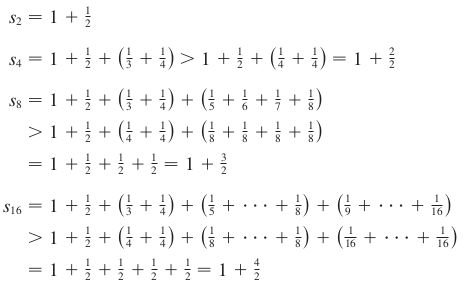
\includegraphics[width=0.7\textwidth]{suma.png}
    %\caption{Suma}
\end{figure}
\end{frame}

\begin{frame}{Preliminar parte IV}
    %\framesubtitle{Borrador}
    \section{Preliminar parte IV}
    En forma similar, $s_{32}>1+\frac{5}{2}$, $s_{64}>1+\frac{6}{2}$, y, en general
    \begin{equation*}
        s_{2^n}>1+\frac{n}{2}
    \end{equation*}
    Esto demuestra que $s_{2^n}\longrightarrow\infty$ cuando $n\longrightarrow \infty$ y por eso $\{s_n\}$ es divergente. Debido a eso, la serie armónica diverge.
\end{frame}

\begin{frame}{Desarrollo}
    %\framesubtitle{Borrador}
    \section{Desarrollo}
    Entonces, sabemos que la sucesión es
    \begin{equation*}
        a_n = \frac{1+n\cdot In(n)}{n^2 +5}
    \end{equation*}
    si nos guiamos por el término dominante del numerador y también por el termino dominante del denominador podemos ver que es similar a 
    \begin{equation*}
        a_n = \frac{1}{n}
    \end{equation*}
\end{frame}

\begin{frame}{Desarrollo parte II}
    %\framesubtitle{Borrador}
    \section{Desarrollo parte II}
    Luego, la serie 
    \begin{equation*}
        \sum_{n=1}^{\infty}b_n = \sum_{n=1}^{\infty}\frac{1}{n}
    \end{equation*}
    es armónica y diverge.
    Por lo que debemos probar que 
    \begin{equation*}
        \lim_{n\rightarrow\infty}\frac{a_n}{b_n}=\infty
    \end{equation*}
\end{frame}


\begin{frame}{Desarrollo parte III}
    %\framesubtitle{Borrador}
    \section{Desarrollo parte III}
    \begin{equation*}
        \lim_{n\rightarrow\infty}\frac{a_n}{b_n}=\lim_{n\rightarrow\infty}\frac{\frac{1+n\cdot In(n)}{n^2+5}}{\frac{1}{n}}
    \end{equation*}
    Realizando lo anterior nos queda
    \begin{equation*}
        \lim_{n\rightarrow\infty}\frac{n(1+n\cdot In(n))}{n^2+5}
    \end{equation*}
    Realizando las operaciones
    \begin{equation*}
        \lim_{n\rightarrow\infty}\frac{n+n^2\cdot In(n)}{n^2+5}
    \end{equation*}
\end{frame}


\begin{frame}{Desarrollo parte IV}
    %\framesubtitle{Borrador}
    \section{Desarrollo parte IV}
    \begin{equation*}
        \lim_{n\rightarrow\infty}\frac{\frac{1}{n}+In(n)}{1+5 \frac{5}{n^2}} = \infty
    \end{equation*}
    Entonces al aplicar la proposición 3 del criterio de comparación por límite, la serie 
    \begin{equation*}
        \sum_{n=1}^{\infty}a_n = \sum_{n=1}^{\infty}\frac{1+n\cdot In(n)}{n^2+5}
    \end{equation*}
    es divergente, pues 
\end{frame}


\begin{frame}{Desarrollo parte V}
    %\framesubtitle{Borrador}
    \section{Desarrollo parte V}
    \begin{equation*}
        \lim_{n\rightarrow\infty}\frac{a_n}{b_n} = \infty
    \end{equation*}
    y
    \begin{equation*}
        \sum_{n=1}^{\infty}b_n = \sum_{n=1}^{\infty}\frac{1}{n}
    \end{equation*}
    es divergente.
\end{frame}


\begin{frame}{Bibliografía}
    %\framesubtitle{Borrador}
    \section{Bibliografía}
    \begin{itemize}
        \item Diapositivas.
        \item Stewart, J. (2011). Single Variable Calculus: Early Transcendentals (7.a ed.). Brooks/Cole Pub Co.
    \end{itemize}
\end{frame}



\end{document}